\section{Editor.\-View.\-Editor\-Window.\-Color\-Property Class Reference}
\label{class_editor_1_1_view_1_1_editor_window_1_1_color_property}\index{Editor.\-View.\-Editor\-Window.\-Color\-Property@{Editor.\-View.\-Editor\-Window.\-Color\-Property}}


A color property.  




Inheritance diagram for Editor.\-View.\-Editor\-Window.\-Color\-Property\-:
\nopagebreak
\begin{figure}[H]
\begin{center}
\leavevmode
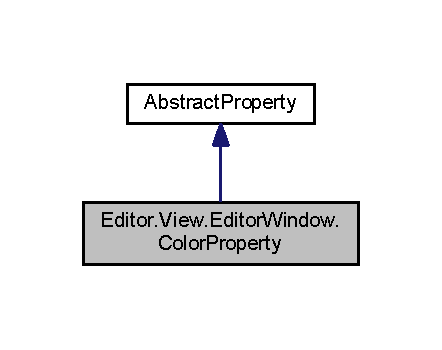
\includegraphics[width=212pt]{class_editor_1_1_view_1_1_editor_window_1_1_color_property__inherit__graph}
\end{center}
\end{figure}


Collaboration diagram for Editor.\-View.\-Editor\-Window.\-Color\-Property\-:
\nopagebreak
\begin{figure}[H]
\begin{center}
\leavevmode
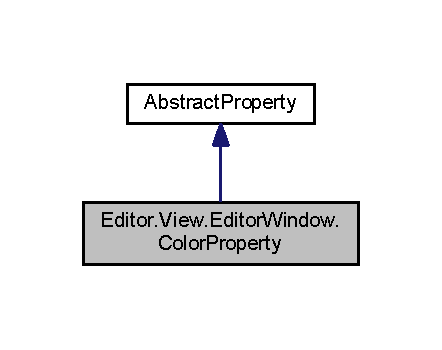
\includegraphics[width=212pt]{class_editor_1_1_view_1_1_editor_window_1_1_color_property__coll__graph}
\end{center}
\end{figure}
\subsection*{Additional Inherited Members}


\subsection{Detailed Description}
A color property. 

Geht, 18.\-12.\-2013. 

Definition at line 20 of file Color\-Property.\-cs.

